\section{Zerocross Detector (Morten og Henrik)}

For at sikre at de enkelte dele af zerocross detectoren virker, realiseres kredsløbet på fumlebræt i flere etaper.\\ 
Først realiseres kredsløbets lavpasfilter, og det konstateres vha. oscilloskop, at det virker som forventet. Der er valgt en $33 k\Omega$ modstand til filteret ($R_{1}$), da dette er den nærmeste værdi, der er tilgængelig. Figur \ref{fig:ZC_Lavpasfilter} viser en måling af signalet efter lavpasfilteret.\\	

\begin{figure}[h]
	\centering
	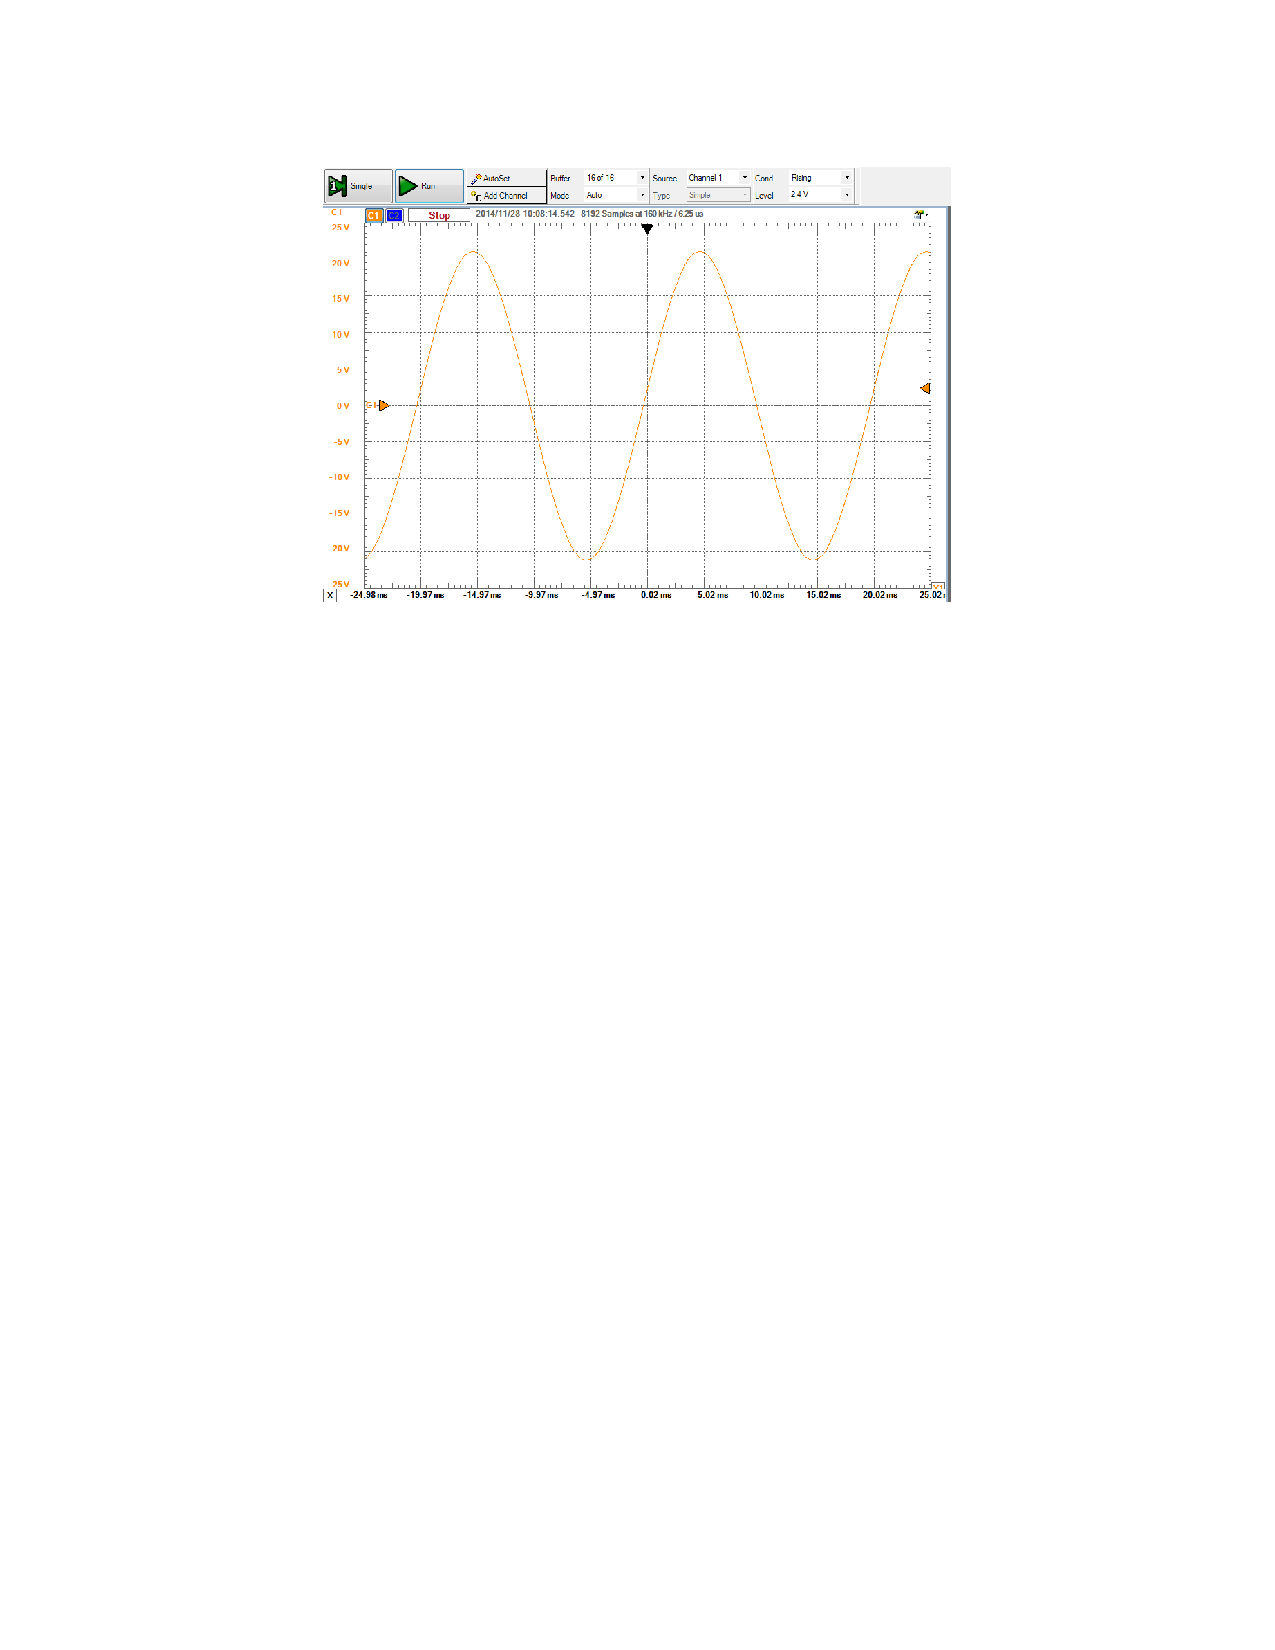
\includegraphics[width={\textwidth},trim=150 500 145 80, clip=true]{../Implementering/billeder/lavpasfilter.pdf}
	\caption{Ren sinus efter lavpasfilter}
	\label{fig:ZC_Lavpasfilter}
\end{figure}

Herefter tilføjes de to dioder ($D_{1}$ og $D_{2}$)\cite{lib:1N4148} på fumlebrættet, og det ses at signalet begrænses som forventet. Signalet er vist på Figur \ref{fig:ZC_Efter_Diode}.\\
\newpage
\begin{figure}[h]
	\centering
	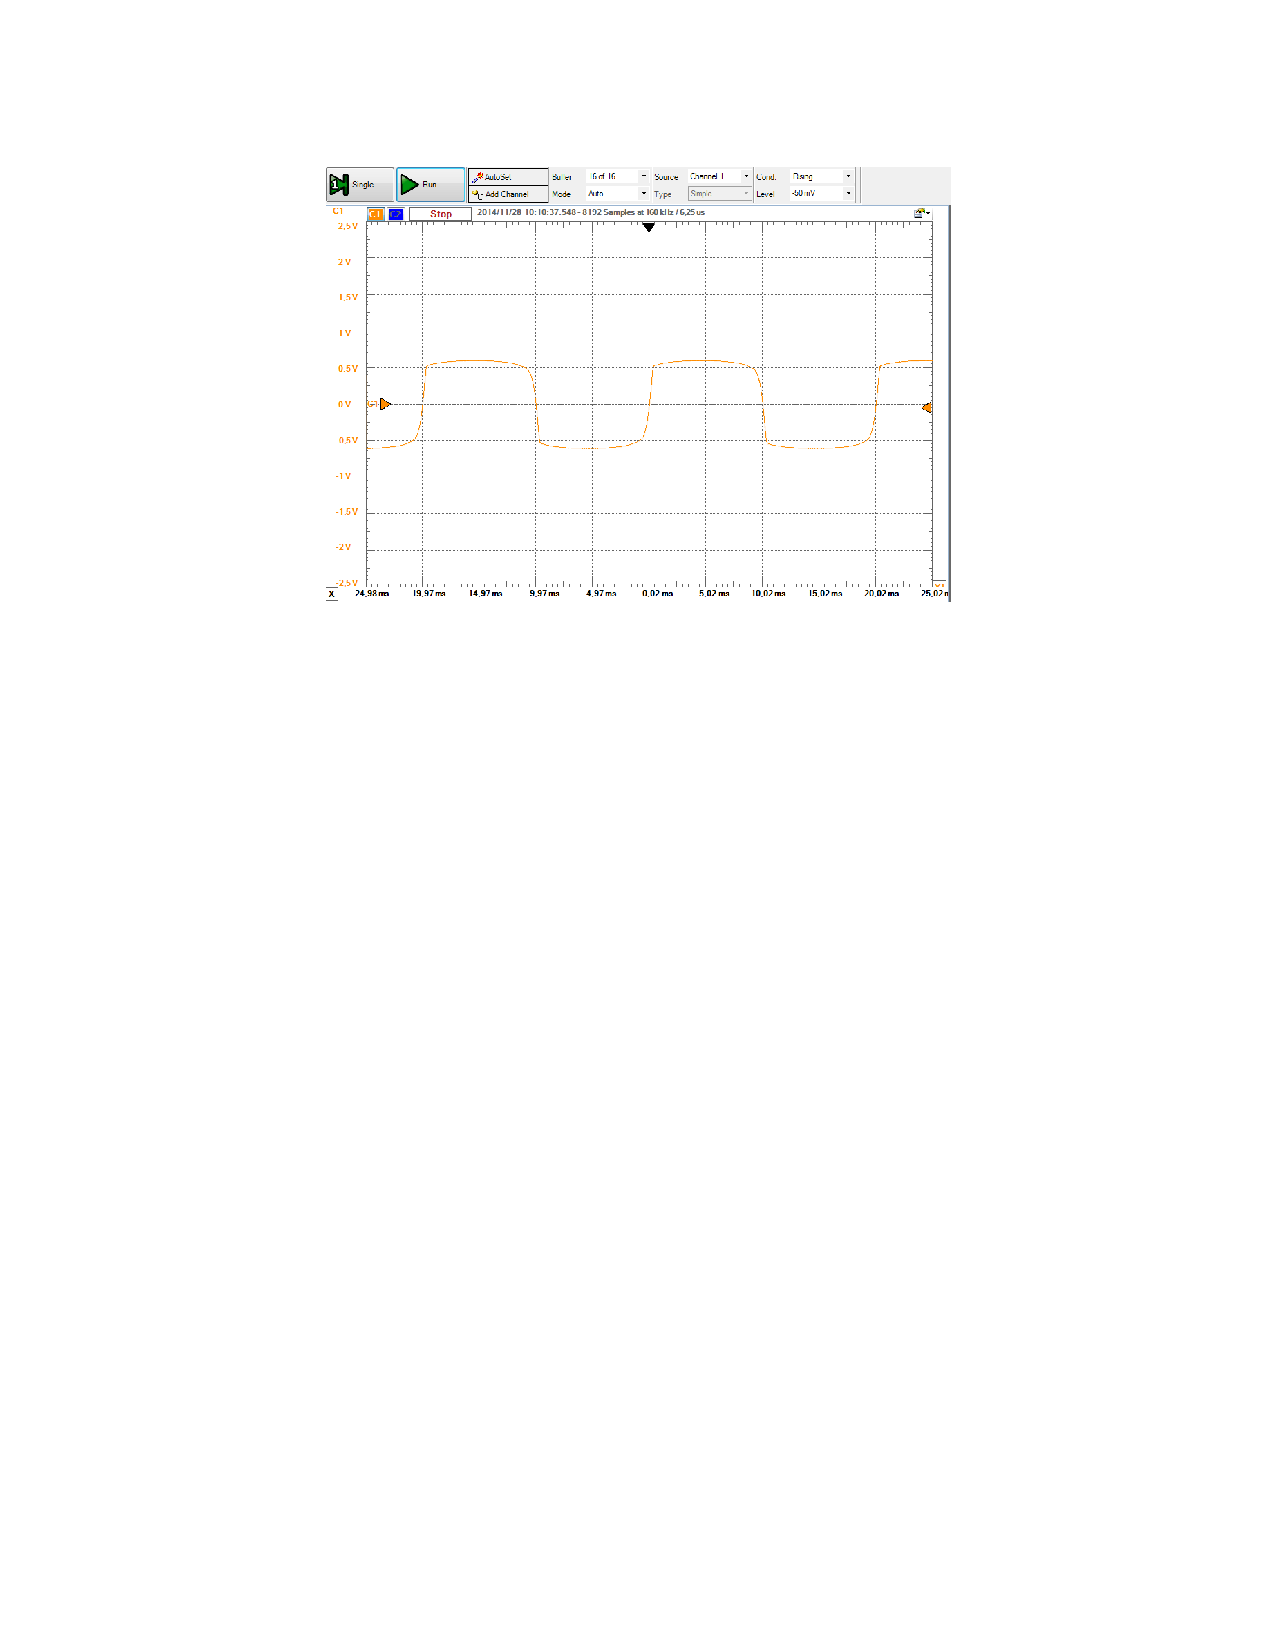
\includegraphics[width={\textwidth},trim=150 505 145 80, clip=true]{../Implementering/billeder/efter_diode.pdf}
	\caption{Dæmpet sinus efter dioder}
	\label{fig:ZC_Efter_Diode}
\end{figure}

Herefter tilføjes komparatoren (TS912)\cite{lib:TS912}, som sammenligner signalet fra Figur \ref{fig:ZC_Efter_Diode} med stel. $R_{2}$ og $R_{3}$ bevirker at der er en hysterese på $200 mV$.\\
Indgange på ubrugte gates er sat til stel. Dioden efter operationsforstærkeren fungerer som forventet.
Udgangssignalet er som ønsket (Figur \ref{fig:ZC_Signal}).\\
 
\begin{figure}[h]
	\centering
	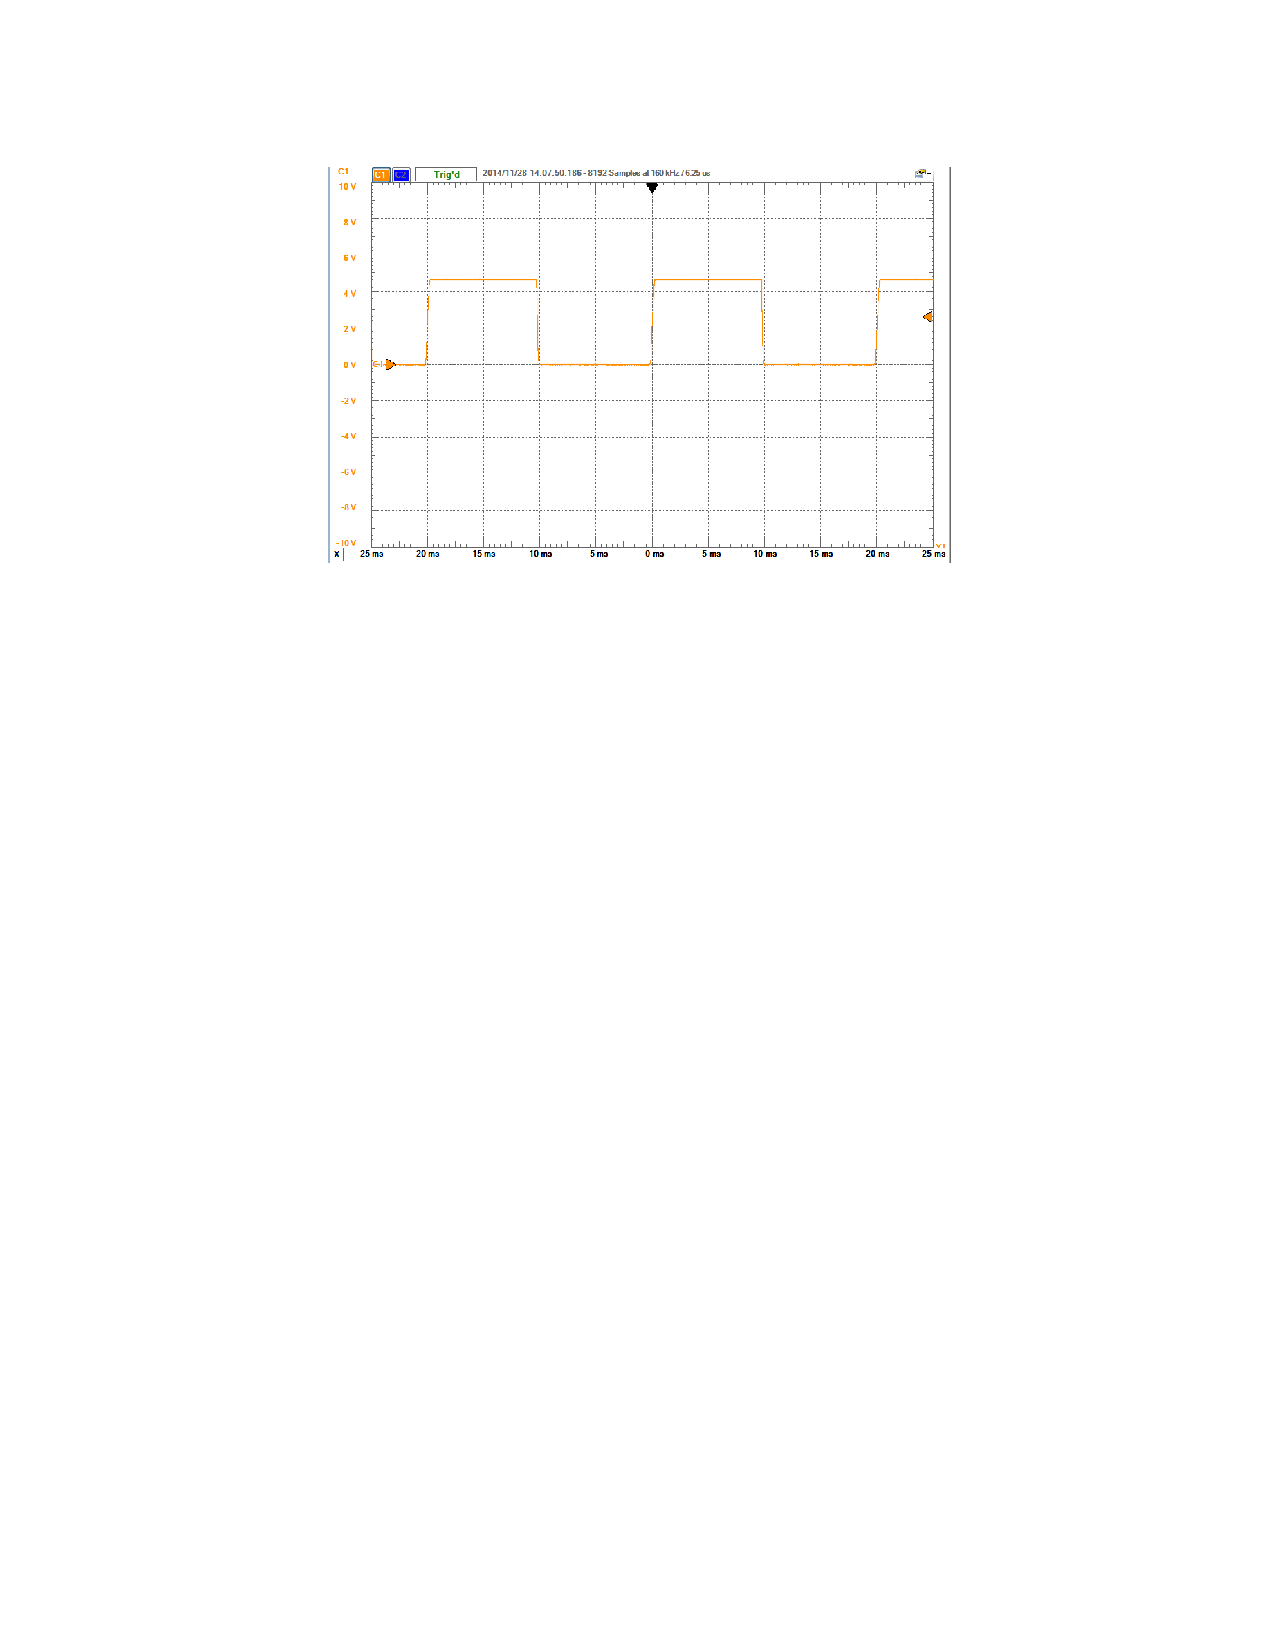
\includegraphics[width={\textwidth},trim=150 520 145 80, clip=true]{../Implementering/billeder/zerocrossdetector.pdf}
	\caption{ZeroCrossDetect signal efter komparator}
	\label{fig:ZC_Signal}
\end{figure}
\newpage